\section{The Large Hadron Collider}
The Large Hadron Collider (LHC) is the proton-proton storage ring operating at CERN and for last 13 years has been the world's highest energy particle collider. The LHC first began operation particles in 2008, but following a magnetic quench incident, it had to be repaired and adjusted, so the first data-taking didn't occur until 2009 \cite{Rossi_2010}. During the 9 years of LHC operation, protons colliding within each of the experiments were increased to larger center-of-mass energies, approaching the design energy of 14TeV. In addition, luminosity has successively been increased, surpassing design luminosity of $1\times10^{34}$cm$^{-2}$s$^{-1}$ in 2018 to reach $2\times10^{34}$cm$^{-2}$s$^{-1}$\cite{CERNnews1}. The overall data recorded in the ATLAS detector totals more than $10^{16}$ collisions. The consistent day-to-day operation of the LHC as well as its strides in increasing the energy and number of collisions produced has led to the most precise measurements of Standard Model constants including the coupling of the Higgs boson to bottom quarks \cite{Aabout_2018_0}, $W$ and $Z$ bosons \cite{Aaboud_2019}, \cite{Aaboud_2018} as well as photons\cite{Aaboud_2018_2} and tau leptons \cite{Aaboud_2019_2}. The LHC has also facilitated searches searches over a wide parameters space, setting confidence level exclusion limits on masses of supersymmetric particles like squarks, gluions and neutralinos \cite{ATLAS-CONF-2019-040}. 

The LHC is set to begin Run 3, in which design center-of-mass energy should be reached, in 2021. Following Run 3, detector upgrades will be made during a long shutdown and then the High-Luminosity LHC (HL-LHC), with unprecedented $10\times$ the luminosity of the LHC, will begin colliding protons in 2027\cite{CERNnews2}. The HL-LHC and its goals will be explained further in \ref{sec:The High-Luminosity LHC and Inner Tracker (ITk)}, suffice to say that LHC-physics is progressing quickly and promises exciting developments in the near future. 

In a brief explanation of the LHC operation, one could begin with the small volume of protons- numbering $\approx 10^{11}$- that is accelerated. Linac 2 is the primary source of protons for CERN accelerators, and has been since the early 1990s \cite{LHCInjector}. This injects protons at 50 MeV into the Proton Synchrotron Booster (PSB) where they are further accelerated to 1.4 GeV. Next they enter the Proton Synchrotron (PS) where the protons are separated into bunches with a spacing of 25 ns and are futher accelerated to 25 GeV before being extracted to the Super Proton Synchrotron (SPS) within which they reach 450 GeV. Finally these bunches of protons enter the LHC and are accelerated to their final energy 6.5 TeV. Linac 2, PSB, PS, and SPS were all operational accelerators prior to being involved in the LHC apparatus, however each had to be majorly upgraded to handle the energy and beam intensity required for LHC collisions \cite{LHCInjector}. 

The LHC basic layout mimics that of the Large Electron Positron collider (LEP) that was housed in the same tunnels prior. Figure \ref{fig:LHClayout} shows the positioning of each experiment on the LHC as well as injection systems and other features. Once proton bunches enter the LHC in two opposing beams they are accelerated with radio frequency (RF) systems. Located at Point 4 in the LHC schematic, the system consists of 16 RF cavities operating at twice the frequency of the SPS injector. RF cavities are metallic chambers containing oscillating electromagnetic fields, in the LHC this oscillation frequency is 400 Mz. The tuning of this frequency ensures that protons of the ideal energy are not accelerated further and simply maintain their maintain their momentum while particles arriving in an RF cavity slightly before or after will be decelerated or accelerated toward the ideal proton energy. This acceleration process can also be used to split beams of protons into discrete bunches, and this is first done with RF cavities in the PS. After proton bunches have circled the LHC approximately 1 million times (15 minutes), peak energy is reached and collisions can commence \cite{radiofrequency}.

\begin{figure}[!h]
        \centering
    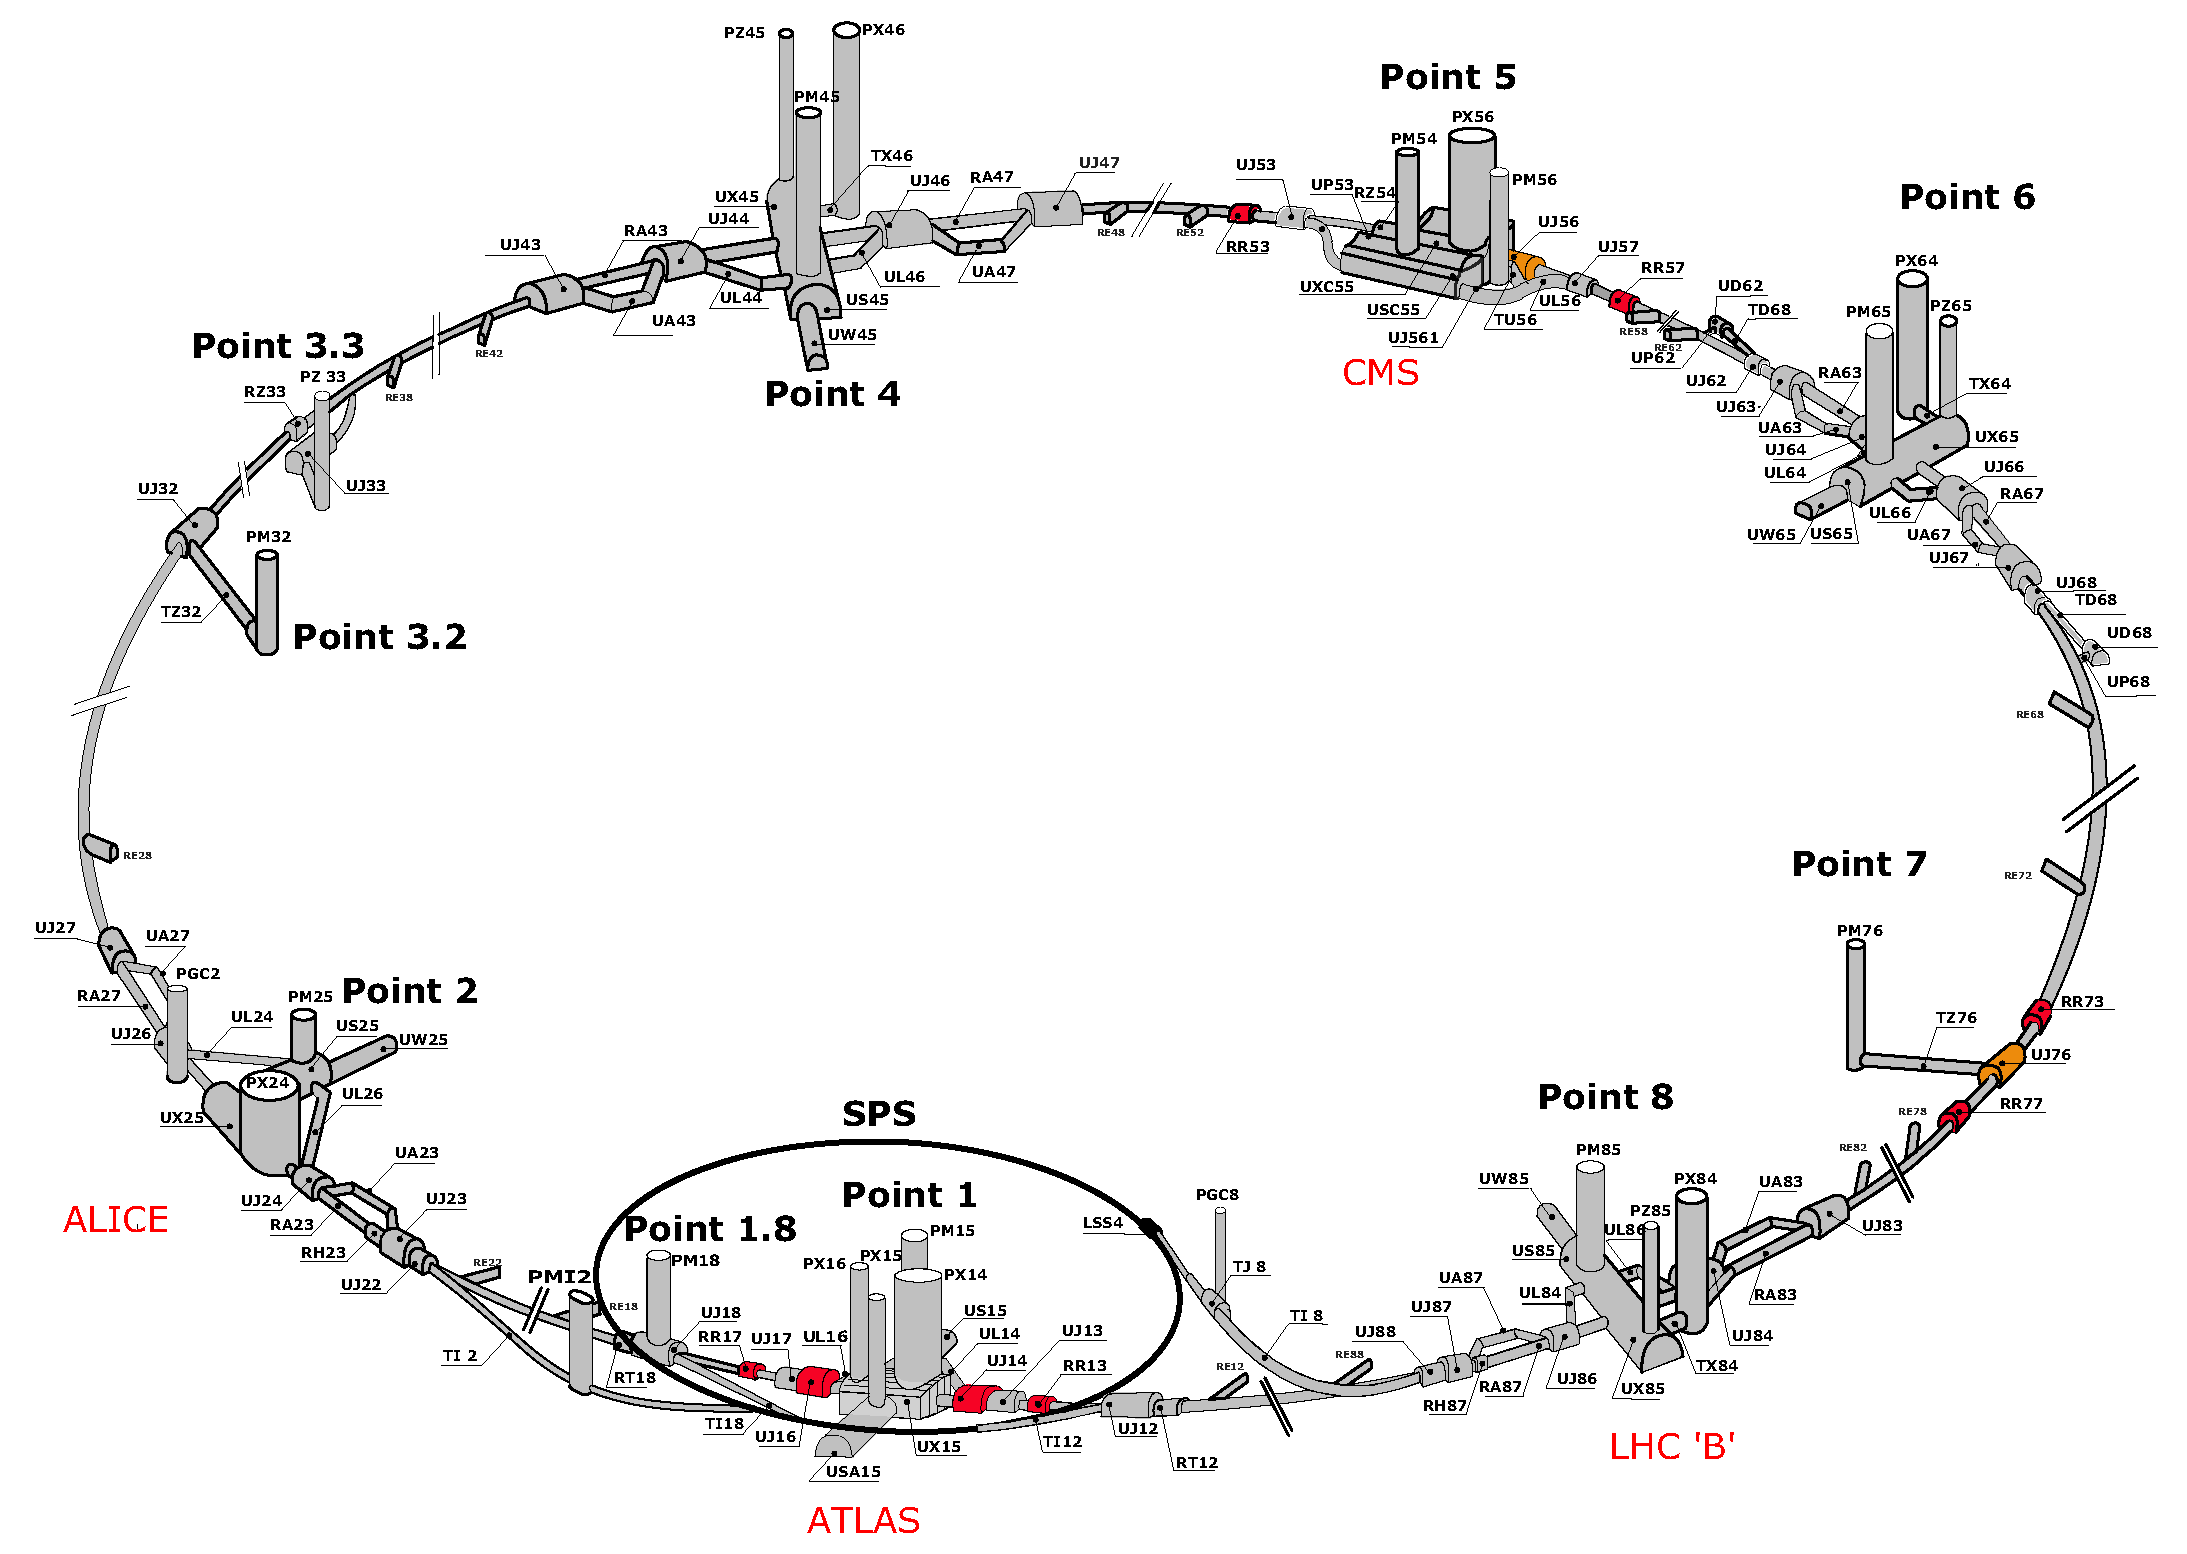
\includegraphics[width=.6\textwidth]{Pictures/LHClayout.PNG}
    \caption{LHC layout \cite{LHCref}}
    \label{fig:LHClayout}
\end{figure}

Superconducting magnets in the LHC in the main dipoles of the create a magnetic field of $\approx 8$T to bend the proton beams into the circlular path of the collider. Figure \ref{fig:dipolemagnet} shows the flux in a dipole cross-section. The oposing direction beamlines are shown centered and the flux is shown to be high (and directionally opposed) in center of each beam. To maintain these fields, the magnets operate at below 1.9K. Pressurized superfluid helium, chosen for its low visosity and high specific heat, cools the dipole magnets. Once the two LHC rings are filled from the SPS, center-of-mass energy of the beams increase until they reach peak energy after about 28 minutes. Finally, proton bunches separated by 25ns collide simultaneously in each detector.  

\begin{figure}[!h]
        \centering
    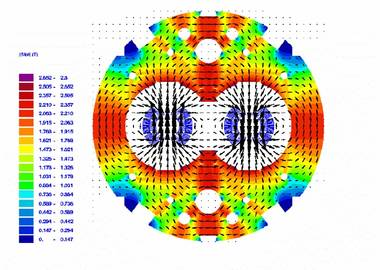
\includegraphics[width=.6\textwidth]{Pictures/dipolemagnet.jpg}
    \caption{ Flux within an LHC dipole cross-section \cite{LHCref}}
    \label{fig:dipolemagnet}
\end{figure}

\section{A Toroidal LHC ApparatuS}
\hspace{20pt} The LHC creates proton-proton collisions at a rate and energy level key for pushing the boundaries of particle physics, but identifying and reconstructing the tracks of such energetic particles decay products is no mean feat. A Toroidal LHC ApparatuS (ATLAS) and the Compact Muon Solenoid (CMS) are multi-purpose detectors built to search for and measure a wide range of particle interactions and properties. Both experiments measured a particle consistentwith the Higgs boson in 2012 and their agreement was a key verification of the discovery. The following sections describe each major component of the ATLAS detector with a focus on their use in the measurement of Higgs$\rightarrow WW \rightarrow e\nu\mu\nu$. 

ATLAS utilizes a coordinate system with its origin at the center of the detector (the ``interaction point") and has a z-axis along the beam pipe. The x-axis points from the interaction point to the center of the LHC ring, and the y-axis points upward. The experiment uses cylindrical coordinates $(r, \phi)$ where $\phi$ is the azimuthal angle around the beam pipe. The pseudorapidity and the transverse momentum are defined in terms of the polar angle $\theta$ as $\eta = -\ln( \tan(\theta/2))$ and $p_T = p\sin\theta$. 
\begin{figure}[!h]
	\centering     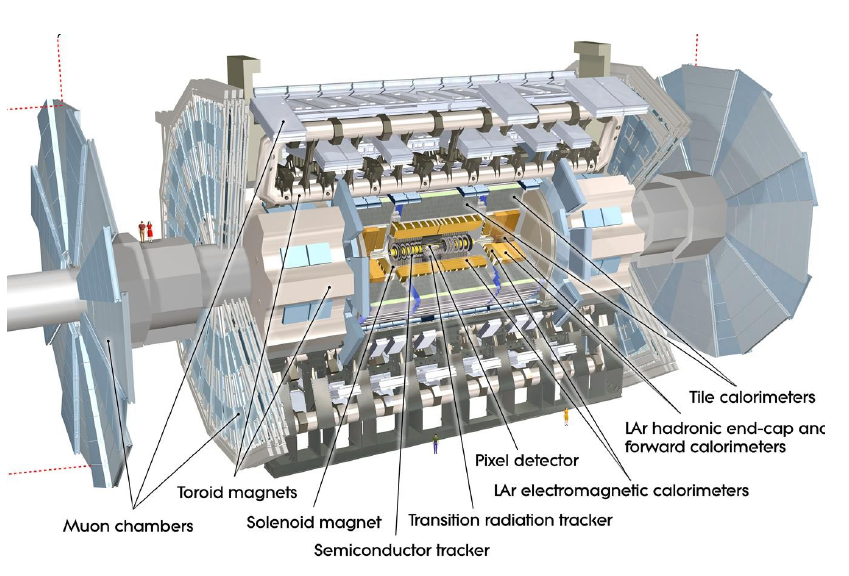
\includegraphics[width=.7\textwidth]{Pictures/ATLASdetector.PNG}
    \caption{Computer-simulated ATLAS detector schematic \cite{detector}}
\end{figure}

\par \hspace{20pt} The Inner Detector (ID) detects charged particles with an $|\eta| < 2.5$ operating in a 2T solenoidal field. It consists of $3$ layers of pixel sensors, $4$ layers of silicon strips, and $72$ straw layers of transition radiation tracker modules. The ID describes particles closest to the interaction point and detects track parameters with great resolution due to high granularity \cite{detector}. 

The ATLAS detector contains 3 superconducting magnet systems- the barrel toroid, 2 end-cap toriods, and a central solenoid. The central solenoid provides a magnetic field for the inner detector while the toroids create a strong magnetic field for for the muon detector. These magnet systems were built to create the largest possible uniform field (for increased momentum resolution on particle tracks) on a large volume enclosing the detector components. They also need to use as little material as possible so as to not unduly influence particles in the detector. The barrel toroids in the barrel and endcap each have 8 coils and creat e a 4T magnetic field while the central solenoid creates a 2T magnetic field in the inner detector. Combined the magnet systems contain $>$100km of superconducting wire which are cooled to working temperatures below 5K \cite{detector}. 

The Muon Spectrometer precision chambers provide muon momentum measurements at a high resolution over a wide range of $p_T$. The MS consists of $3$ layers of Monitored Drift Tube chambers covering $|\eta| < 2.7$ and an inner layer of Cathode Strip Chambers with $|\eta| > 2.0$. In addition, it includes trigger chambers that contain $3$ layers of Resistive Plate Chambers ($|\eta| < 1.05$) and $3$ layers of Thin Gap Chambers ($1.05 < |\eta| < 2.4$). As the outermost subdetector, the MS provides precise muon momentum measurements along the muon trajectory and the muon chambers are located with a precision of under $60$ $\mu m$. The MS also contains a system of three superconducting toroidal magnets each with eight coils providing a magnetic field with a bending integral of up to $6$ Tm \cite{detector}. 

Calorimeters provide detailed information about the energy deposited as particles pass through. Electromagnetic calorimeters detect and halt the motion of electrons and photons while the hadronic calorimeter does the same for hadrons. Muons and neutrinos are able to pass through the calorimeters to the MS. The electromagnetic and hadronic calorimeter, made of liquid Argon and scintillating tiles, respectively, are able to pass information from the location of energy deposits to the muon reconstruction algorithm \cite{detector}. 

\section{The High-Luminosity LHC and Inner Tracker (ITk)}
Though the LHC succeeded in one of its crucial goals of discovering the Higgs boson in 2012, its continuous operation at higher energy and luminosity has led to more rigorous measurements of the Higgs as well as searches for new physics beyond the Standard Model. The LHC has been the leading high energy collider in terms of person power, energy, and scale for over a decade and will continue to be extremely important for understanding theoretical questions in the future. While more data collection is planned in Run-3 starting in 2021 \textcolor{red}{??}, new colliders and detectors take decades to design, develope and build, so the plans for the collider to take it's place is well underway. The High Luminosity LHC will operate at an LHC-level energy (14TeV) and begin data-taking in 2026. The HL-LHC will begin with $5-7\times$ the luminosity of the LHC and will have a design luminosity of $10\times$ the LHC, or $12.6\times10^{-34}$cm$^{-2}$s$^{-1}$. This huge increase in number of collisions requires massive upgrades to the LHC including new, 11-12T superconducting magnet systems, compact superconducting caivities for beam rotation and phase control, and new technology beam collimation \cite{HL-LHC Yellow Paper}. This massive undertaking has been underway for many years already and has involved laboratories all over the world.

Just as the LHC had to be re-designed and built to create higher luminosity, so too do all the experiments on the LHC have to be redesigned to be able to interpret so many more collisions per second. The detectors must be built to withstand more radiation, as the increased collision rate also means a high radiation rate especially closest to the beamline. They also have to provide greater granularity to be able to reconstruct tracks with good enough resolution that individual tracks can be discriminated. Finally, they have to be able to deal with increased pile-up. Pile-up is caused by high numbers of collisions occuring at each bunch crossing. When there is a large amount of pile-up it becomes difficult to trace which particle tracks come from the same interaction point. Finally, the increased data in and of itself creates a complex problem for the detectors to solve, as briefly discussed previously, the trigger system must quickly choose which collision events may hold interesting events and store these. When there are more events happening near simultaneously these systems must make these decisions in real-time. New algorithms to speed up this process are necessary when there are an order of magnitude more events to sort through.

Detectors for high energy colliders are not built often- expensive and time-consuming to design and test, they're made to last at least a decade. I was lucky to have the opportunity to work on ATLAS detector research and development during a year I worked at Brookhaven National Laboratory during my Ph.D. and though my thesis isn't directly related to this work, it was formative and extremely interesting, so I'll touch on this work in the next section. Because I worked on the new ATLAS inner detector for the HL-LHC (termed Inner Tracker or ITk) I will just discuss this sub-detector and the particular role I played in its assembly.

\subsection{Inner Tracker (ITk)}
The Inner Tracker is planned to be an all-silicon detector that will completely replace the current Inner Detector.  While the current ID has been extremely successful during Runs 1 and 2 (and will certainly continue to be in Run 3), it does not have to capacity to withstand the radiation and pile-up conditions of the HL-LHC. The ITk is designed to operate for 10 years under instantaneous luminosity of 7.5$\times10^{-34}$cm$^{-2}$s$^{-1}$ with 25ns between bunch crossings. This will result in 1,000 fb$^{-1}$ and average pile0up up to $<\mu>=200$ \cite{ITktech}. The current solenoid magnet will remain in the detector with a 2T magnetic field. The ITk will consist of an innermost section with silicon pixels and an outtermost section of silicon strips. The pixel detector will contain four barrel layers and six forward region disks, while the strip detector will contain five barrel layers and seven disks. The rapidity range matches the coverage of the Muon Spectrometer with $|\eta|<2.7$, this layout is shown in \ref{fig:ITklayout}. 
\begin{figure}[!h]
        \centering
    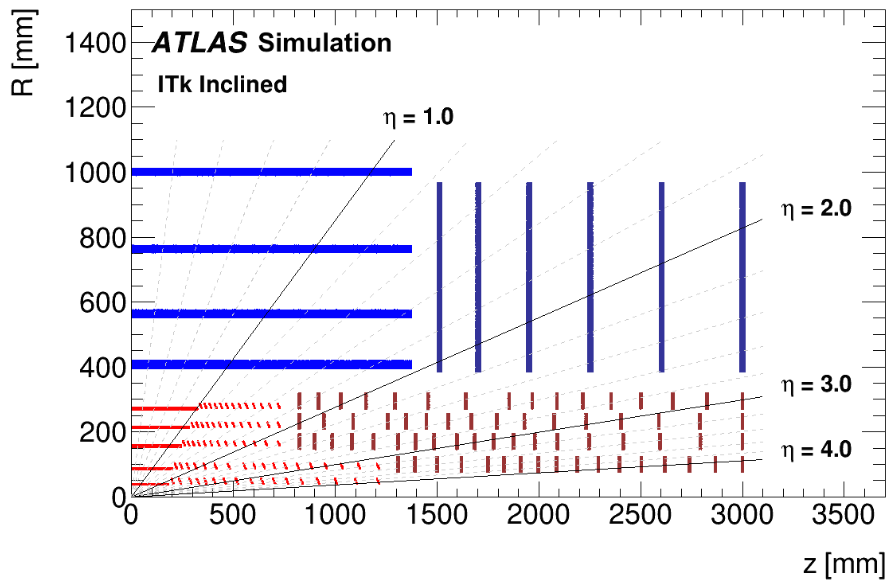
\includegraphics[width=.6\textwidth]{Pictures/ITklayout.png}
    \caption{ ITK layout as defined in Technical Design Report \cite{ITktech}}
    \label{fig:ITKlayout}
\end{figure}

\subsubsection{Building ITk Strip barrel staves}
I spent 1.5 years of my Ph.D. at Brookhaven National Laboratory (partially funded through a SCGSR Fellowship) and was able to make key contributions to the ITk Strip barrel stave assembly effort. The goal of stave assembly is to precisely calibrate specified positions for silicon modules on carbon fiber stave cores and then glue them in place within a 25$\mu$m tolerance. Brookhaven National Laboratory is responsible for assembly of half off all ITk staves (~200) and the accurate assembly is necessary for the ITk to reduce uncertainty on track positions and to ensure a symmetric detector. At Brookhaven, I was tasked with co-creating a stave assembly software system through LabView to automatically calibrate required module positions, apply a layer of adhesive gel, and guide the user to accurately place the module into its specified location. This project was highly collaborative and evolved further after I left the laboratory, but the overall process remains unchanged.

The basic design of the Inner Tracker for both barrel and endcap components is the same - a carbon fiber core (containing titanium cooling pipes) is covered on each side with co-cured kapton service tapes. The carbon fiber core is designed to reduce overall radiation length and the similar design in the barrel and endcap adds to simplicity. Silicon modules are glued to stave cores. Similar radial silicon strip detectors have been used previously in both ATLAS and CMS but never covering so much fiducial area. The modules consist of one silicon sensor and one or two low-mass PCB's (hybrid) which host ASICs. Module design has optimized producibility and low cost while maintaining readout goals. Overall module design is the same in barrel and endcap regions, while strip lengths and geometries vary. Compnents of a short-strip barrel module are shown in \ref{fig:module}.
\begin{figure}[!h]
        \centering
    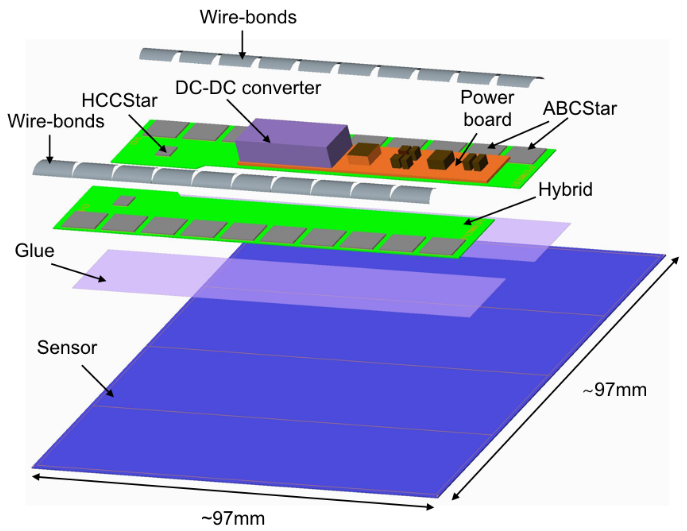
\includegraphics[width=.4\textwidth]{Pictures/ITkmodule.png}
    \caption{Short-strip barrel module components \cite{ITktech}}
    \label{fig:module}
\end{figure}
 
Each barrel stave core needs to be "loaded" with 14 modules, as shown in the assembled electrical prototype in \ref{fig:stave}. The placement of these modules needs to be accurate to below 25$\mu$m so that the detector is symmetrical and ITk models accurately demonstrate particle track positions. After the detector is assembled and commisioned tests will be done with laser alignment to understand the exact positioning of the modules and staves but any module positioning out of specification will have adverse affects on track resolution during operation. 

\begin{figure}[!h]
        \centering
    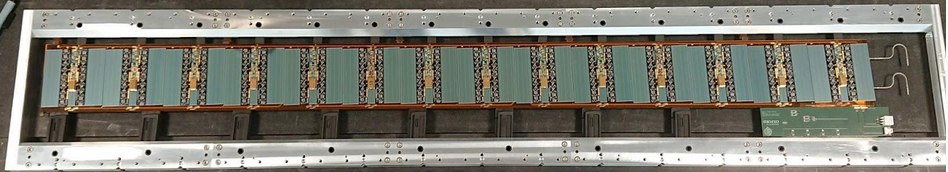
\includegraphics[width=.8\textwidth]{Pictures/electricalstave.png}
    \caption{Electrical stave prototype at BNL}
    \label{fig:stave}
\end{figure}

Brookhaven National Laboratory is one of two sites resposible for assembling barrel staves and their assembly procedures have been tested with the production of numerous prototypes including a thermomechanical double-sided stave and a fully operational electrical stave. The thermomechanical prototype was later used for various thermal tests, including IR imaging (documented in the next section), and the electrical stave is currently undergoing tests for read-out. Stave assembly is composed of three main parts- system calibration, module placement, and  survey of results. 

Staves at BNL are assembled on a granite table housing an Aerotech XYZ Stage (accurate to the micron level). The stage is equiped with a 10-megapixel camera that gives real-time feedback to a nearby computer and a glue dispenser. The stave assembly software system is implemented by a user who interacts with the LabView GUI and monitors progress. The stave is fixed to optical rails drilled into the table. In order to accurately place modules in their correct positions a series of calibrations need to be completed including camera calibrations to test the optimal working point, focus, and pixel-to-micron conversion. Next, the position of the stave with relation to the XYZ stage needs to be calibrated. Tranforming coordinates of the XYZ stage to that of the stave and so specified coordinates for modules atop their carbon fiber cores requires locating a fixed point on the stave core as well as the angle of the stave relative to the XYZ stage. Pattern matching algorithms find the exact locations of particular features on the stave core and allow calculation of required positions for all modules based on specifications. Once specified module positions are calculated, calibrations are complete and it's time to apply glue and afix modules. 


Next, an epoxy (SE4445) is loaded into the glue dispenser on the XYZ-stage which is connected to a vaccuum controlled by the LABView software system. The epoxy is automatically dispensed in lines to cover $\approx$ 60\% of area under the module and then the module is lifted with a custom-made "pick-up" tool which uses a vacuum applied to module corners to hold the module in place and move it to the needed position along the optical rails. Then, using real-time feedback from the software system and its pattern matching algorithm the user is directed on how to finetune the positon of the module using knobs on the "pick-up" tool. Markings etched in the silicon sensor at each corner which are used to position the module accurately. The output of the module alignment GUI is shown in \ref{modulealignment}. When the module is within specifications it is lowered into position above the epoxy and held in place for 24 hours until the glue has completely dried.

\begin{figure}[!h]
        \centering
    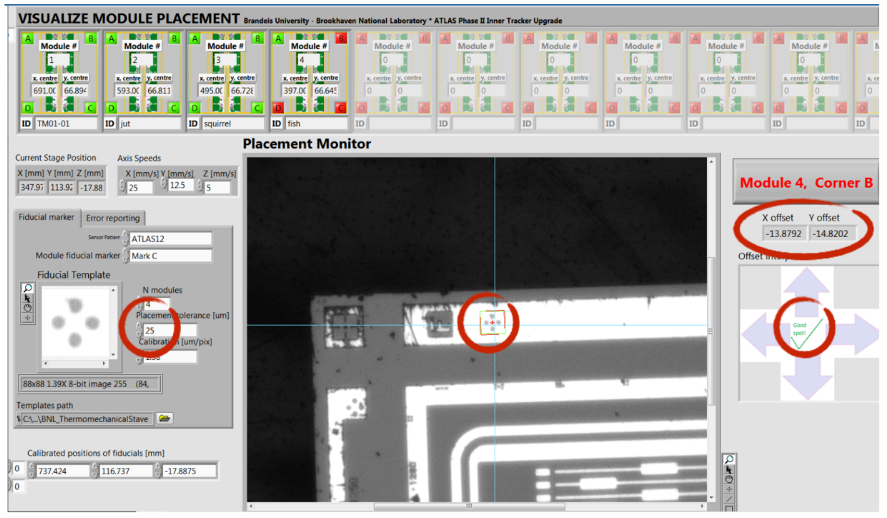
\includegraphics[width=.6\textwidth]{Pictures/labviewscreen.png}
    \caption{GUI interface showing etched marking on module corner located in real-time to guide user on how to adjust module position}
    \label{fig:modulealignment}
\end{figure}

Finally, after the glue has set, a final survey of module positions (taken by using pattern matching to find the positions of etched markings on each corner) is taken. These results are saved into an ITk database and checked for any biases. After module placement on the stave is complete, it is moved to another station in the lab for wirebonding so that all data from the modules can be read-out to stave-wide electronics and then moved off detector. The module assembly system has worked quite well at placing modules accurately for all prototypes, achieving specification requirements for almost all modules. Results of the first prototype stave module placement are shown in \ref{fig:placementresults}. While a few module corners are slightly out of the ideal range, the majority are well within specifications. While building prototypes, some issues and inefficiencies were found and corrected. New hardware, like an improved glue system temperature monitoring were also added during prototype assembly. The methods described continue to be in use now and will be utilized for the production of 200 ITk staves at BNL. 

\begin{figure}[!h]
        \centering
    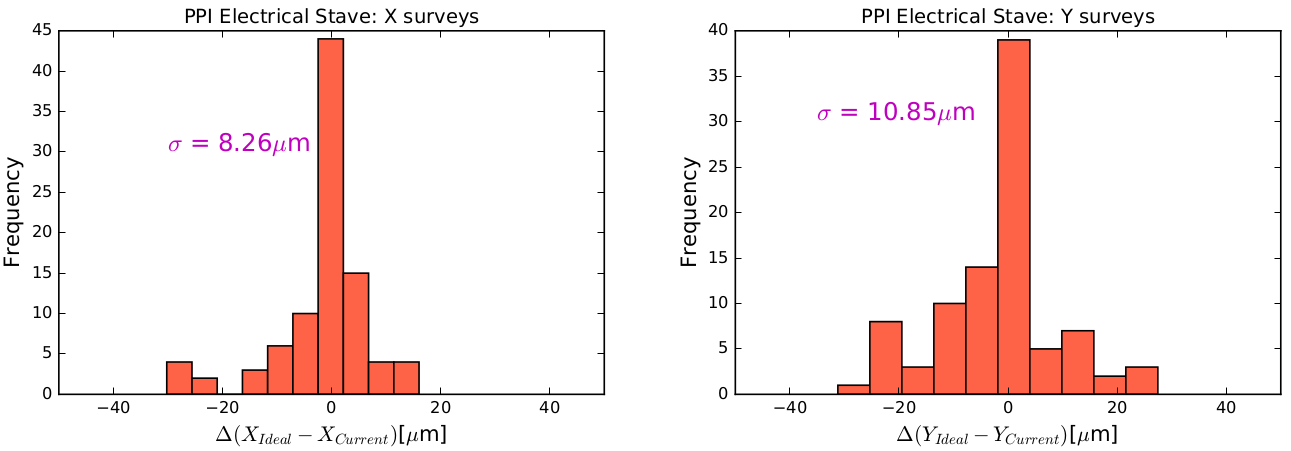
\includegraphics[width=.8\textwidth]{Pictures/placementresults.png}
    \caption{Histograms show difference between ideal and final position of each module corner. Left shows difference from specification in X and right in Y.}
    \label{fig:placementresults}
\end{figure}

\subsubsection{IR Testing ITk Strip barrel staves}
The first full US stave prototype is the thermo-mechanical stave, built in the summer of 2017.  Building this stave was the first test of the stave assembly procedure and methods and the results showed success. This stave was also assembled to test the thermal and mechanical properties of a fully loaded barrel stave. Multiple tests were done including thermal studies (using thermistors and IR imaging), thermal cycling and thermal shock tests, mechanical studies, and bending tests. I will give a short summary on IR imaging tests, as these were another focus of my time at BNL. First, the thermo-mechanical stave consists of 13 modules mounted on each side. The modules used are thermo-mechanical, which means that instead of the usual readout chips their hybrids have copper traces to mimic the power dissipation and location of the chips. The powerboard can vary the TM hybrid power dissipation of each module individually. In addition, these modules each have three thermistors- one of the DC-DC converter, and one on each of two hybrids. The stave is powered by a custom End-of-Substructure (EoS) card which is attached to a RaspberryPi and Arduino and can power on or off each module.  

Thermal testing of barrel staves had a few main goals: first, to compare with Finite Element Analysis simulations and so test that all temperature trends are as we expect, to make sure that individual modules- and their slightly modified assembly methods- don't exhibit abnormal thermal behavior, and finally to check that loaded staves can cope with potential issues they might face during operation. I will highlight a few key results which demonstrate that each of these goals have been accomplished. 

Thermal measurements were taken both through the mounted thermistors on each module and through IR imaging. IR imaging provides information about the entirety of the loaded stave, rather than at just a few module positions so provides a more complete picture. The loaded stave was spray-painted black with a high emissivity, low conductivity black paint since silicon is transparent to the IR camera spectrum (8-14$\mu$m). In order to image the entire stave core, the IR camera was attached to rails above and pulled at a constant speed with an external motor as it recorded video. The frames were then stitched together into one image. A section of the painted stave is shown in \ref{fig:paintedstave}.  

\begin{figure}[!h]
        \centering
    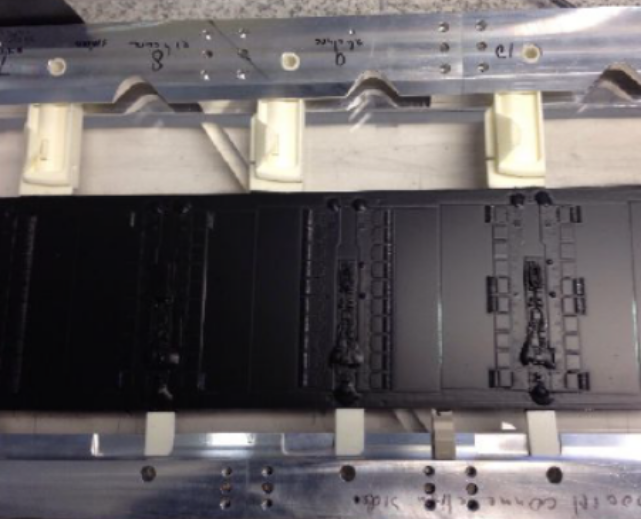
\includegraphics[width=.4\textwidth]{Pictures/paintedstave.png}
    \caption{Portion of the thermo-mechanical stave after spray-painted for increased emissivity}
    \label{fig:paintedstave}
\end{figure}

FEA simulations for the thermal performance of a stave were completed by Prof. Graham Beck at QMUL. These calculations quickly became intractable if convection was included, so conditions of the stave and coolant were adjusted such that convective constributions were minimal, or the total electrical power and power absorbed into the coolant were identical. At BNL we adjusted the coolant temperature until we saw this convective power minimization, then recorded module temperatures under these conditions. These results were compared to the FEA simulations by averaging hybrid temperatures recorded through IR imaging and recording NTC thermistor readings. These comparisons are shown in \ref{fig:FEAcompare}. The measurements show very good agreement with FEA calculations, within 5\% of the expected values.

\begin{figure}[!h]
        \centering
    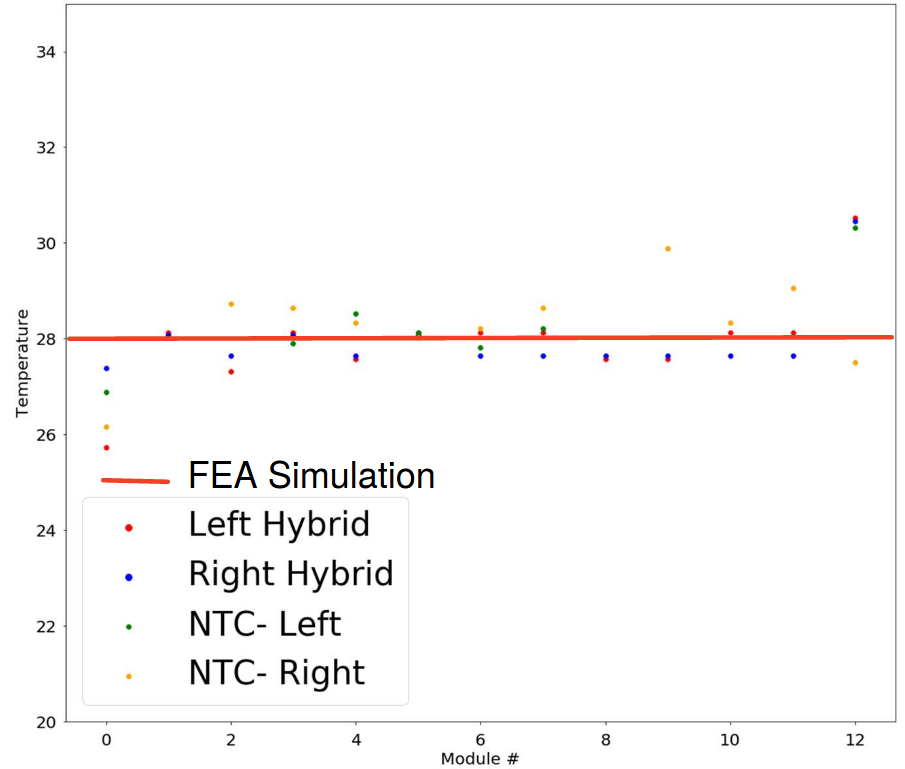
\includegraphics[width=.4\textwidth]{Pictures/FEAcompare.png}
    \caption{IR measurements, NTC thermistor measurements, and FEA simulations for the TM stave are compared. Agreement with expected within 5\%}
    \label{fig:FEAcompare}
\end{figure} 

During module assembly some slight variations were tested including varying glue thickness below modules and glue curing time, and FEAST versions. Module with these variations were noted and compared to those without at varying coolant temperatures and output power settings. Overall, no significant differences in module temperature change was observed for any of these assembly modifications. Fully loaded stave thermal properties are thus robust to assembly modifications like these. Figure \ref{fig:IRimagetotal} shows a full IR image of the fully loaded stave. It's clear that there are no obvious module-to-module variations in silicon, hybrid, or FEAST temperature. The module sensors increase in temperature as they get closer to the EoS, which is expected since it dissipates power to the stave.

\begin{figure}[!h]
        \centering
    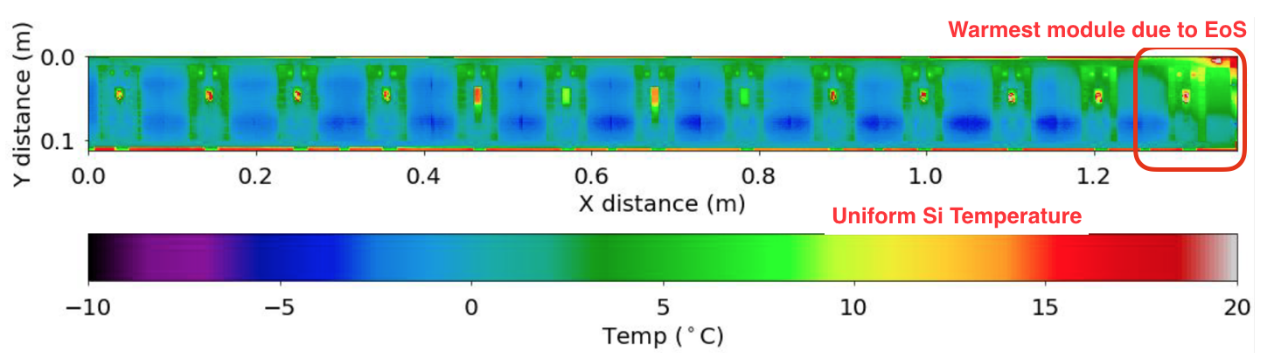
\includegraphics[width=.8\textwidth]{Pictures/IRimagetotal.png}
    \caption{IR image of fully loaded thermo-mechanical stave}
    \label{fig:IRimagetotal}
\end{figure} 
 
The thermo-mechanical stave was pushed to limits beyond what we would expect loaded staves to encounter during operation and never exhibited unexpected behavior. Thermal cycles, thermal shocks and bend tests showed the loaded stave robust to intense temperature variation and that the carbon fiber core is as stiff as it was prior to loading. Another test was how neighboring modules would perform if one module malfunctioned and went offline. Figure \ref{fig:moduleoff} shows temperature of each module when one of them (fourth to the left) turns off. The rest of the modules continue to operate normally and temperature changes from the unpowered module don't propagate very far. The second image in the figure shows the reverse of the stave when a module is powered off (fourth from the right). The temperature effects are greater directly below than adjacent to- which is expected. 

\begin{figure}[!h]
        \centering
    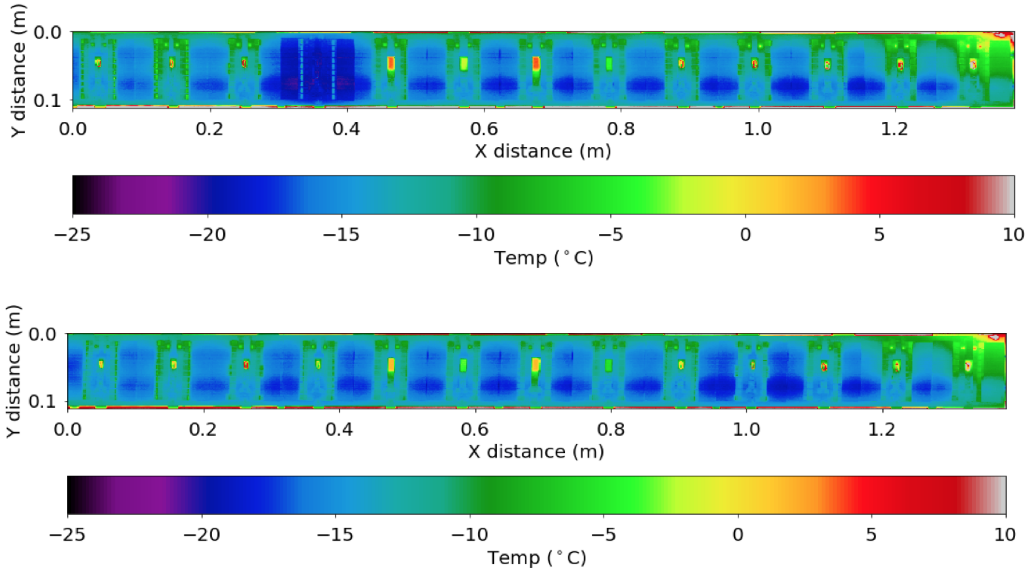
\includegraphics[width=.7\textwidth]{Pictures/moduleoff.png}
    \caption{IR image of fully loaded thermo-mechanical stave}
    \label{fig:moduleoff}
\end{figure}

